%A good requirement is:
%*Correct
%*Unambiguous (all statements have exactly one interpretation)
%*Complete (where TBDs are absolutely necessary, document why the information is unknown, who is responsible for resolution, and the deadline)
%*Consistent
%*Ranked for importance and/or stability
%*Verifiable (avoid soft descriptions like “works well”, “is #user frndly”; use concrete terms and specify measurable #quantities)
%*Modifiable (evolve the Requirements Specification only via a #formal change process, preserving a complete audit trail of #changes)
%*Does not specify any particular design
%*Traceable (cross-reference with source documents and spawned documents).




\chapter{Requirement specification}

\section{Version history}
\begin{table}[H]
\begin{tabular}{|c|p{9cm}|c|c|}
\hline
Version & Description & Author & Date\\
\hline
0.1 & Initial draft & JK & 21/12-13\\
\hline
0.2 & Figure 2.1 updated, minor functional requirement changes, Central data unit and sensor node description added. & JK & 09/01-14\\
\hline
0.3 & General system description added & NG & 09/01-14\\
\hline
\end{tabular}
\end{table}

\section{Purpose}
The purpose of this document is to present a detailed description of the Charcot foot prevention system. It thoroughly outlines and specifies the features, interfaces, purpose of the system as well as under which constraints the system will operate under.\\
The intended audience of the document is the developers, the supervisor and Delta.\\
The requirements of the system may only be changed after a review meeting with the group and stakeholders.\\

\section{Scope}
These specifications are limited to the bachelor's project, and not the whole potential system as described in the "Project description" provided from delta.\\

\section{References}
$\bullet$ Project description

\section{Glossary}
\begin{table}[H]
\centering
\begin{tabular}{|p{4cm}|p{7cm}|}
\hline
Term & Definition\\ \hline
CDU & Abbreviation of "Central Data Unit", a key component in the system. \\ \hline
Delta & The company which this project is made in collaboration with.\\ \hline
BOM & Build Of Material abbreviation\\ \hline
\end{tabular}
\end{table}

\section{General description}

\subsection{General System}
\begin{figure}[H]
	\centering
	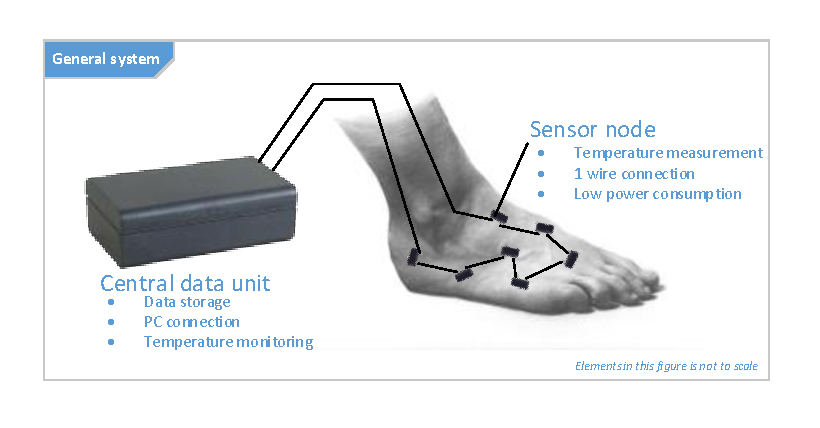
\includegraphics[width=1\textwidth]{billeder/GeneralSystem}
	\caption{General System}
\end{figure}

\subsection{System description}
Et device der skal påmonteres foden på en person der er disponeret til at udvikle Charcotfod. Devicet skal ud fra temperatur og aktivitetsniveau finde ud af om der er en fare for overbelastning. Hvis dette er tilfældet skal brugeren advares.

\subsubsection{Central data unit description}
The central data unit communicates with the sensor nodes to collect data from each node. This data is stored on the CDU's memory with a time stamp and sensor node identifier.\\
The CDU can transfer the data to a computer. This communication can be wired or wireless but this may be implemented solely as a feature for this project and not the final product, which is an excluded feature for this project.

\subsubsection{Sensor node description}
The sensor node is in general a generic sensor which contains two functionalities. It contains the custom 1-wire protocol and it can measure data. This measurement can be temperature, accelerometer value etc. The nodes gets both power and communication via. one wire in and is then daisy chained to the next sensor and so forth until the wire ends in the CDU again. This helps minimize wires in the insole/sock and simplifies the system. 

\subsection{Constraints}
\textit{Currently none.}
\subsection{Dependencies}
\textit{Currently none.}

%\subsection{Prototype af UI eller GUI}

%\subsection{Beskrivelse af UI eller GUI}

\section{Functional requirements}
Below is listed all functional requirements to the system.\\
\textbf{\large{Priority definitions}}\\
The following definitions are intended as a guideline to prioritize requirements.
\begin{itemize}[noitemsep,nolistsep]
\item Priority 1 - This is a "Need to Have" either defined by law or of most importance of the project.
\item Priority 2 - This requirement is if high importance and will be of great benefit for the system
\item Priority 3 - This requirement will be great to have but not important
\item Priority 4 - This requirement is purely "Nice-to-have" and will not be considered unless there is time to spare.
\end{itemize}


\subsection{Actors of the system}

\subsubsection{Primary actors}

\begin{table}[H]
	\centering
	\begin{tabular}{|l|p{7cm}|}
	\hline
	Actor name & Central data unit \\ \hline
	Type & Primary \\ \hline
	Description & The Central data unit is the main actor of the system. The Central data unit contacts sensors and manage data. It consists of a microcontroller and some memory for data. \\ \hline
	\end{tabular}
\end{table}

\begin{table}[H]
	\centering
	\begin{tabular}{|l|p{7cm}|}
	\hline
	Actor name & Patient \\ \hline
	Type & Primary \\ \hline
	Description &  The patient set the system to run and initiates data extraction from the CDU.\\ \hline
	\end{tabular}
\end{table}

\subsubsection{Secondary actors}

\begin{table}[H]
	\centering
	\begin{tabular}{|l|p{7cm}|}
	\hline
	Actor name & Sensor \\ \hline
	Type & Secondary \\ \hline
	Description & The sensor actor consists of a sensor, a microcontroller and a powercontrol unit. It responds to messages initiated by the central data unit.\\ \hline
	\end{tabular}
\end{table}

\begin{table}[H]
	\centering
	\begin{tabular}{|l|p{7cm}|}
	\hline
	Actor name & Computer \\ \hline
	Type & Secondary \\ \hline
	Description & The computer can extract data from the central data unit. It is not intended as a control unit but mostly just for demonstration purposes. \\ \hline
	\end{tabular}
\end{table}




\subsection{Use Case diagram}
Below is shown the use case diagram.
\begin{figure}[H]
\centering
\includegraphics*[width=.7\textwidth]{billeder/UseCase_vector}
\label{usecase_fig}
\caption{Use case diagram}
\end{figure}

\subsection{Use Cases}

\subsubsection{Set system to normal operation}

\begin{table}[H]
	\centering
	\begin{tabular}{|l|p{10cm}|}
	\hline
	Goal 							& To set the system to normal operatio.n \\ \hline
	Initialisation 					& The Patient initiates the use case. \\ \hline
	\multirow{2}{*}{Actors} 		& Patient \\ 
									& CDU \\ \hline
	Reference 						& Get data from sensor \#X \\ \hline
	\# of concurrent events 		& 1 \\ \hline
	Prerequisite  					& The patient connect the sensors to the port on the CDU. \\ \hline
	Post condition 					& The system is set to normal operation. \\ \hline
	\multirow{5}{*}{Main Scenario} 	& 1. The patient clicks the  "ON"-button. \\
	& 2. The CDU checks if the sensors are connected.\\
	& 3. The CDU scans for sensors within address range and stores the addresses along with a sensor numbers.\\ 
	& 4. The CDU checks if the memory is responding.\\
	& 5. The CDU reads which memory space is being used from the memory.\\ \hline
	\multirow{6}{*}{Exceptions} & 2a. The sensors are not connected \\ 
								& - The CDU indicates an error and stops operation.\\											& 2b. There is no response from any sensor\\
								& - The CDU indicates an error and stops operation. \\
								& 4c. The memory is not responding\\
								& - The CDU indicates an error and stops operation. \\ 
								\hline
	Priority					& 1\\\hline
	\end{tabular}
\end{table}

\subsubsection{Get data from sensor \#X}
\begin{table}[H]
	\centering
	\begin{tabular}{|l|p{10cm}|}
	\hline
	Goal 							& Collect data from a sensor. \\ \hline
	Initialisation 					& The CDU runs a cycle and each cycle collects data from each sensor. The CDU then initiates the get data from sensor when it is time. \\ \hline
	\multirow{2}{*}{Actors} 		& CDU \\ 
									& Sensor \\ \hline
	\multirow{2}{*}{Reference}		& Set system to normal operation \\ 
									& Store data \\\hline
	\# of concurrent events 		& 1 \\ \hline
	Prerequisite  					& The usecase "Set system to normal operation" must have been completed. \\ \hline
	Post condition 					& Data has been acquired from sensor \#X \\ \hline
	\multirow{5}{*}{Main Scenario} 	& 1. The CDU determines which sensor to collect data from. \\
	& 2. The CDU contacts the sensor with the correct address and a command to send data back.\\
	& 3. The sensor responds with the data.\\ 
	& 4. The CDU validates if the data is within reasonable range. \\
	& 5. Initiates use case "Store data".\\ \hline
	\multirow{8}{*}{Exceptions} & 2a. The CDU cannot send data \\ 
								& - The CDU indicates an error and stops operation.\\											& 3b. There is no response from sensor\\
								& - The CDU indicates an error and continues operation. \\
								& 4c. The data is out of reasonable range.\\
								& - The CDU reinitiates the use case "Collect data from a sensor". \\ 
								& 4d. The data is out of reasonable range 3 times in a row with the same sensor. \\
								& - The CDU indicates an error and continues operation.\\ \hline
	Priority					& 1\\\hline
	\end{tabular}
\end{table}

\subsubsection{Store data}
\begin{table}[H]
	\centering
	\begin{tabular}{|l|p{10cm}|}
	\hline
	Goal 							& Save the data on memory \\ \hline
	Initialisation 					& The CDU initiates this use case once "Get data from \#X" has been completed. \\ \hline
	\multirow{1}{*}{Actors} 		& CDU \\ \hline
	Reference 						& Get data from sensor \#X. \\ \hline
	\# of concurrent events 		& 1 \\ \hline
	Prerequisite  					& The use case "Get data from sensor \#X" must have been completed. \\ \hline
	Post condition 					& Data has been stored on memory \\ \hline
	\multirow{4}{*}{Main Scenario} 	& 1. The CDU initiates the save data sequence because new data has been acquired from a sensor. \\
									& 2. The CDU gives the data a timestamp and the correct sensor number.\\
									& 3. The CDU transfers the data to the memory.\\ 
									& 4. The CDU reads the data again from the memory to ensure the data has been stored correctly. \\ \hline
	\multirow{4}{*}{Exceptions} & 3a. The CDU cannot transfer data. \\ 
								& - The CDU indicates an error and stops operation.\\											& 4a. The data was not stored correctly. \\
								& - The CDU reinitiates the "Store data" use case.\\\hline
	Priority					& 1\\\hline
	\end{tabular}
\end{table}

\subsubsection{Extract data from CDU}
\begin{table}[H]
	\centering
	\begin{tabular}{|l|p{10cm}|}
	\hline
	Goal 							& Extract the data from CDU.\\ \hline
	Initialisation 					& The patient connects the CDU to a computer. \\ \hline
	\multirow{3}{*}{Actors} 		& Patient \\ 
									& CDU \\
									& Computer \\\hline
	Reference 						& None \\ \hline
	\# of concurrent events 		& 1 \\ \hline
	Prerequisite  					& The system has been collecting data.\\ \hline
	Post condition 					& The data has been transferred to a computer. \\ \hline
	\multirow{4}{*}{Main Scenario} 	& 1. The patient disconnects the CDU from the sensors and connects it to the computer. \\
									& 2. The patient opens the program to transfer data.\\
									& 3. The patient sets up the program and sends the transfer command.\\ 
									& 4. The CDU responds with the data. \\ \hline
	\multirow{4}{*}{Exceptions} & 4a. The CDU does not respond. \\ 
								& - The CDU and computer are not connected correctly.\\											& 4b. The CDU responds "There is no data". \\
								& - There is not data on the CDU to respond with.\\\hline
	Priority					& 3\\\hline
	\end{tabular}
\end{table}

\section{Non functional requirements}
Below is listed all non-functional requirements. \\

\subsection{General requrements}
\begin{table}[H]
\begin{tabular}{p{10cm} p{2cm}}
$\bullet$ The system should be simple and not be of any discomfort of the patient. & \\
$\bullet$ The system should be small enough to have on a belt or similar and in a sock or shoe. &\\
$\bullet$ BOM Price & 40€\\
\end{tabular}
\end{table}


\subsection{Temperature sensor requirements}

\subsubsection{Functionality Requirements}
\begin{table}[H]
\begin{tabular}{p{8cm} p{5cm}}
$\bullet$ Accuracy: & <$0.5^o$C\\
$\bullet$ Update rate: & min. once per CDU cycle\\
$\bullet$ Lifespan: & > 3 year\\
\end{tabular}
\end{table}

\subsubsection{Hardware Requirements}
%Krav til hardware (if any)\\
\begin{table}[H]
\begin{tabular}{p{8cm} p{2cm}}
$\bullet$ Power consumption: & <0.05W\\


\end{tabular}
\end{table}


\subsubsection{Software Requirements}
%Krav til software (if any)\\
\begin{table}[H]
\begin{tabular}{p{8cm} p{2cm}}
$\bullet$ Timer: & Yes\\


\end{tabular}
\end{table}


\subsubsection{External interfaces}
\begin{table}[H]
\begin{tabular}{p{8cm} p{2cm}}
$\bullet$ 1 wire protocol: & Yes\\
$\bullet$ Wires in: & 1\\
$\bullet$ Wires out: & 1\\
\end{tabular}
\end{table}

\subsection{Central data unit requirements}

\subsubsection{Functionality Requirements}
\begin{table}[H]
\begin{tabular}{p{8cm} p{2cm}}
$\bullet$ Cycle\footnotemark: & 1 min\\
\end{tabular}
\end{table}
\footnotetext{In a cycle the CDU will collect data once from all sensors}
\subsubsection{Hardware Requirements}
%Krav til hardware (if any)\\
\begin{table}[H]
\begin{tabular}{p{8cm} p{2cm}}
$\bullet$ Power consumption: & <0.5W \footnotemark \\
$\bullet$ Memory: & >1MB\footnotemark\\
$\bullet$ Real time clock: & Yes\\
\end{tabular}
\end{table}
\footnotetext{Sensor supply excluded}
\footnotetext{Or at least enough to store data for an entire day}

\subsubsection{Software Requirements}
%Krav til software (if any)\\
\begin{table}[H]
\begin{tabular}{p{8cm} p{2cm}}
$\bullet$ Save entries must contain: &Sensor nr. \\
~ 									&Temperature. \\
~									&Timestamp. \\


\end{tabular}
\end{table}


\subsubsection{External interfaces}
\begin{table}[H]
\begin{tabular}{p{8cm} p{2cm}}
$\bullet$ 1 wire protocol: & Yes\\
$\bullet$ CDU to computer interface: & Yes\\
\end{tabular}
\end{table}

\subsection{Project requirements}

\subsubsection{Documentation}
\begin{itemize}
\item Engelsk
\item SysML
\end{itemize}

\subsubsection{Technologies and tools}
\begin{itemize}
\item Matlab
\item Maple/Mathcad
\item Microsoft Visio 2010/2013
\item TortoiseSVN
\item TeXmaker
\end{itemize}

\subsubsection{Misc}
\begin{itemize}
\item Report is written in LaTeX.
\end{itemize}

